% Variant C -- Multi-Core NN Inference (architecture concept)
\label{ch:mcnn}

%=============================================================
% History
%=============================================================
\section{History}

\begin{table}[H]
\caption{History}
\label{tab:mcnnhistory01}
\centering
\begin{tabularx}{\textwidth}{|X |X |X |}
  \hline
  \multicolumn{3}{|l|}{History} \\
  \hline
  \multicolumn{1}{|l}{Target Spec.} & \multicolumn{1}{l}{Current version : 0.1, 2026-11-06} & \multicolumn{1}{l|}{Author: A. Siggelkow}\\
  \multicolumn{1}{|l}{ } & \multicolumn{1}{l}{Previous version : ---} & \multicolumn{1}{l|}{ }\\
  \hline
  \hline
  Paragraph (in previous version) & Paragraph (in current version) / date & Subjects (major changes since last revision) \\
  \hline
  \hline
  \multicolumn{3}{|l|}{Current Chapter Version: C0.1; Date: 2026-11-06} \\
  \hline
  & \ref{ch:mcnn} / 2026-11-06 & First draft of the architecture concept for Variant~C (AS, Claude) \\
  \hline
\end{tabularx}
\end{table}

%=============================================================
% Purpose and scope
%=============================================================
\section{Purpose and Scope}
\label{sec:mcnnscope}

This chapter describes \textbf{Variant~C}, a planned third chip variant of
the \aschip project in addition to Variant~A (\texttt{RV\_NoPipeline}) and
Variant~B (\texttt{RV\_PipelineCacheFwd}), see
Table~\ref{tab:asChipVariants}.
Variant~C is a small multi-core system for the \textbf{inference of
quantised neural networks} (NN) such as multi-layer perceptrons (MLP) and
small convolutional networks (CNN).

\textbf{Status:} architecture concept. No part of Variant~C is implemented
yet. All sizes, addresses and register maps in this chapter are
\emph{proposals}; values marked TBD are decided during implementation.

The guiding ideas are:
\begin{itemize}
  \item \textbf{Compute in the instruction set, not in the core count.}
    A custom SIMD instruction \texttt{nn.dot8} performs 8 int8
    multiply-accumulates (MAC) per instruction using the existing 64-bit
    data path. It contributes more performance than additional cores.
  \item \textbf{Software-managed memory instead of caches.}
    The data access pattern of NN inference is known at compile time.
    The worker cores therefore use tightly coupled memories (TCM) filled by
    a DMA controller instead of data caches. No hardware cache coherence
    is required anywhere in the system.
  \item \textbf{Reuse of existing blocks.}
    The pipeline core \texttt{cc\_cpupipefwd}, the I-Cache, the QSPI
    controller, the ICU, the shared interrupt register block
    \texttt{as\_irq\_peripheral} and the peripheral kernels are reused.
\end{itemize}

Variant~C is a teaching and demonstrator chip. It is not intended to
compete with dedicated NN accelerators; the extension path towards such an
accelerator is shown in Section~\ref{sec:mcnnroadmap}.

%=============================================================
% Requirements
%=============================================================
\section{Requirements}
\label{sec:mcnnreq}

Requirements follow IEEE\;29148 terminology:
\textit{shall} = mandatory, \textit{should} = recommended,
\textit{may} = optional.
Each identifier has the form \textbf{MCNN-\textit{CAT}-\textit{NNN}}
with the category codes of Table~\ref{tab:mcnnReqCat}.

\begin{table}[H]
\caption{Variant C Requirements -- Category Codes}
\label{tab:mcnnReqCat}
\centering
\begin{tabularx}{\textwidth}{|l |X|}
  \hline
  Category Code & Scope \\
  \hline
  \hline
  SY & System structure \\
  \hline
  CO & CPU core and instruction set \\
  \hline
  ME & Memories \\
  \hline
  IC & Interconnect \\
  \hline
  DM & DMA controller \\
  \hline
  SN & Synchronisation and inter-processor interrupts \\
  \hline
  IF & External interfaces \\
  \hline
  VE & Verification \\
  \hline
\end{tabularx}
\end{table}

\begin{longtable}{|p{0.15\textwidth} |p{0.45\textwidth} |p{0.32\textwidth}|}
\caption{Variant C Requirements}
\label{tab:mcnnReq}\\
  \hline
  ID & Requirement & Notes / Rationale \\
  \hline
  \hline
\endfirsthead
  \hline
  ID & Requirement & Notes / Rationale \\
  \hline
  \hline
\endhead
  MCNN-SY-001 &
    The system \textit{shall} contain one control core (\textbf{Core0},
    hart~0) and four worker cores (\textbf{W1}\ldots\textbf{W4},
    harts~1\ldots4). &
    Core0: boot, host communication, scheduling.
    Workers: NN kernels. \\
  \hline
  MCNN-SY-002 &
    The number of worker cores \textit{should} be a top-level parameter
    (\texttt{NR\_WORKERS}, 1\ldots4). &
    Allows a single-worker configuration for bring-up and area reduction. \\
  \hline
  MCNN-SY-003 &
    The system \textit{shall not} require hardware cache coherence. &
    Coherence is guaranteed by software and the DMA controller
    (Section~\ref{sec:mcnnmem}). \\
  \hline
  MCNN-CO-001 &
    All cores \textit{shall} implement RV64I plus the
    \textbf{M} extension (MUL, MULH, MULHSU, MULHU, MULW, DIV, DIVU, REM,
    REMU, DIVW, DIVUW, REMW, REMUW). &
    Required by the C compiler for index arithmetic and by the
    requantisation step. \\
  \hline
  MCNN-CO-002 &
    Multiplication and division \textit{may} be implemented as multi-cycle
    iterative units stalling the pipeline
    (MUL $\leq$ 34 cycles, DIV $\leq$ 66 cycles). &
    The NN inner loop uses \texttt{nn.dot8} (MCNN-CO-003); the 64-bit
    multiplier is used only once per output value. \\
  \hline
  MCNN-CO-003 &
    The worker cores \textit{shall} implement the custom instruction
    \texttt{nn.dot8} (Section~\ref{subsec:mcnndot8}). Core0
    \textit{should} implement it. &
    8 MAC per instruction. \\
  \hline
  MCNN-CO-004 &
    All cores \textit{shall} implement the CSR \texttt{mhartid}
    (\texttt{0xF14}) with a value fixed by a parameter. &
    The same binary runs on all workers and selects its work by hart ID. \\
  \hline
  MCNN-CO-005 &
    All cores \textit{shall} evaluate the machine software interrupt
    (\texttt{mip.MSIP}, bit~3) in addition to \texttt{mip.MEIP}. &
    Inter-processor interrupts (MCNN-SN-002).
    Currently only \texttt{irq\_ext\_i[7]} (MEIP) is evaluated. \\
  \hline
  MCNN-CO-006 &
    The reset vector \textit{shall} be a per-hart parameter. &
    Core0 boots from Flash, workers from their ITCM. \\
  \hline
  MCNN-CO-007 &
    The cores \textit{should} implement \texttt{WFI}; a NOP implementation
    is permitted in the first version. &
    Idle workers wait for an IPI; a real WFI allows clock gating later. \\
  \hline
  MCNN-ME-001 &
    Each worker \textit{shall} have a private instruction TCM
    (\textbf{ITCM}) and a private data TCM (\textbf{DTCM}) and
    \textit{shall not} have an I-Cache or D-Cache. &
    Deterministic 1-cycle access; no tag arrays; no coherence. \\
  \hline
  MCNN-ME-002 &
    Each DTCM \textit{shall} consist of two independently accessible banks. &
    Double buffering: the core computes on one bank while the DMA fills the
    other (Section~\ref{subsec:mcnnpingpong}). \\
  \hline
  MCNN-ME-003 &
    Core0 \textit{shall} have an I-Cache for execute-in-place (XIP) from the
    NOR Flash and a DTCM; it \textit{shall not} have a D-Cache. &
    Reuses the existing I-Cache; the D-Cache would create a coherence problem
    with the DMA controller. \\
  \hline
  MCNN-ME-004 &
    The system \textit{shall} contain a shared SRAM organised in at least
    two banks. &
    Holds weights, activations and messages; banking avoids serialising
    five masters on one port. \\
  \hline
  MCNN-ME-005 &
    Accesses of the cores to the shared SRAM and to the peripherals
    \textit{shall} be uncached. &
    Consequence of MCNN-SY-003. \\
  \hline
  MCNN-ME-006 &
    Every TCM \textit{shall} be visible under a hart-local address (alias)
    and under a unique global address. &
    Local: identical binary on all workers.
    Global: target for DMA and Core0. \\
  \hline
  MCNN-IC-001 &
    The memory interconnect \textit{shall} be AMBA AXI4 including the write
    channels (AW, W, B). &
    Variant~B uses read channels only. \\
  \hline
  MCNN-IC-002 &
    The peripherals \textit{shall} be connected via AMBA AXI4-Lite through
    an AXI4-to-AXI4-Lite bridge. &
    Replaces Wishbone; see Section~\ref{subsec:mcnnperbus}. \\
  \hline
  MCNN-IC-003 &
    The interconnect \textit{shall} arbitrate each slave round-robin among
    the requesting masters. &
    No starvation of a worker. \\
  \hline
  MCNN-IC-004 &
    A core access to its own TCM \textit{shall} have priority over a DMA
    access to the same TCM bank. &
    The DMA waits (AXI wait states); the pipeline never stalls on a local
    TCM access because of DMA. \\
  \hline
  MCNN-DM-001 &
    The DMA controller \textit{shall} provide one channel per hart
    (\texttt{NR\_WORKERS}+1 channels). &
    By convention channel~$h$ is programmed by hart~$h$; no channel
    allocation protocol is needed. \\
  \hline
  MCNN-DM-002 &
    Each channel \textit{shall} support 2D transfers (rows, row length,
    source stride, destination stride). &
    Tiles of weight matrices and feature maps are 2D. \\
  \hline
  MCNN-DM-003 &
    Each channel \textit{shall} raise an interrupt on completion and on
    error, using \texttt{as\_irq\_peripheral} (\texttt{irqs\_yes\_no}\,=\,0). &
    Same register model as GPIO/UART. \\
  \hline
  MCNN-SN-001 &
    The mailbox block \textit{shall} provide at least 8 hardware
    semaphores with test-and-set read semantics. &
    Mutual exclusion without the A extension. \\
  \hline
  MCNN-SN-002 &
    The mailbox block \textit{shall} allow every hart to set and clear the
    MSIP interrupt of every hart. &
    Inter-processor interrupts (IPI). \\
  \hline
  MCNN-SN-003 &
    After reset the workers \textit{shall} be held inactive until Core0
    releases them via the mailbox register \textbf{MBOX0\_HART\_RUN}. &
    Core0 loads the ITCMs before the workers fetch their first
    instruction. \\
  \hline
  MCNN-IF-001 &
    Variant~C \textit{shall} reuse QSPI0 for the NOR Flash (boot code and
    NN weights) and UART0 for control and debug. & \\
  \hline
  MCNN-IF-002 &
    Variant~C \textit{should} contain a host interface \textbf{HOSTIF0}
    for an external USB FIFO bridge
    (FT232H-type synchronous 245 FIFO, 8 bit). &
    Purely digital, 10--40\,MB/s; see Section~\ref{sec:mcnnext}. \\
  \hline
  MCNN-IF-003 &
    PCIe \textit{shall not} be part of the ASIC implementation. &
    Requires a SerDes PHY (analogue hard IP) that is not available in the
    target process. An FPGA prototype may use a PCIe hard IP. \\
  \hline
  MCNN-VE-001 &
    The ISS scoreboard of the cocotb environment \textit{shall} be extended
    by the M extension and \texttt{nn.dot8}. &
    Section~\ref{sec:mcnnverif}. \\
  \hline
  MCNN-VE-002 &
    The NN results of the chip \textit{shall} be compared bit-exactly with a
    reference model (Python/NumPy, integer arithmetic). & \\
  \hline
\end{longtable}

%=============================================================
% System overview
%=============================================================
\section{System Overview}
\label{sec:mcnnoverview}

Figure~\ref{fig:mcnnblock} shows the block diagram of Variant~C.
Red connections are AXI4, green connections AXI4-Lite.

\begin{figure}[H]
\centering
\resizebox{\textwidth}{!}{%
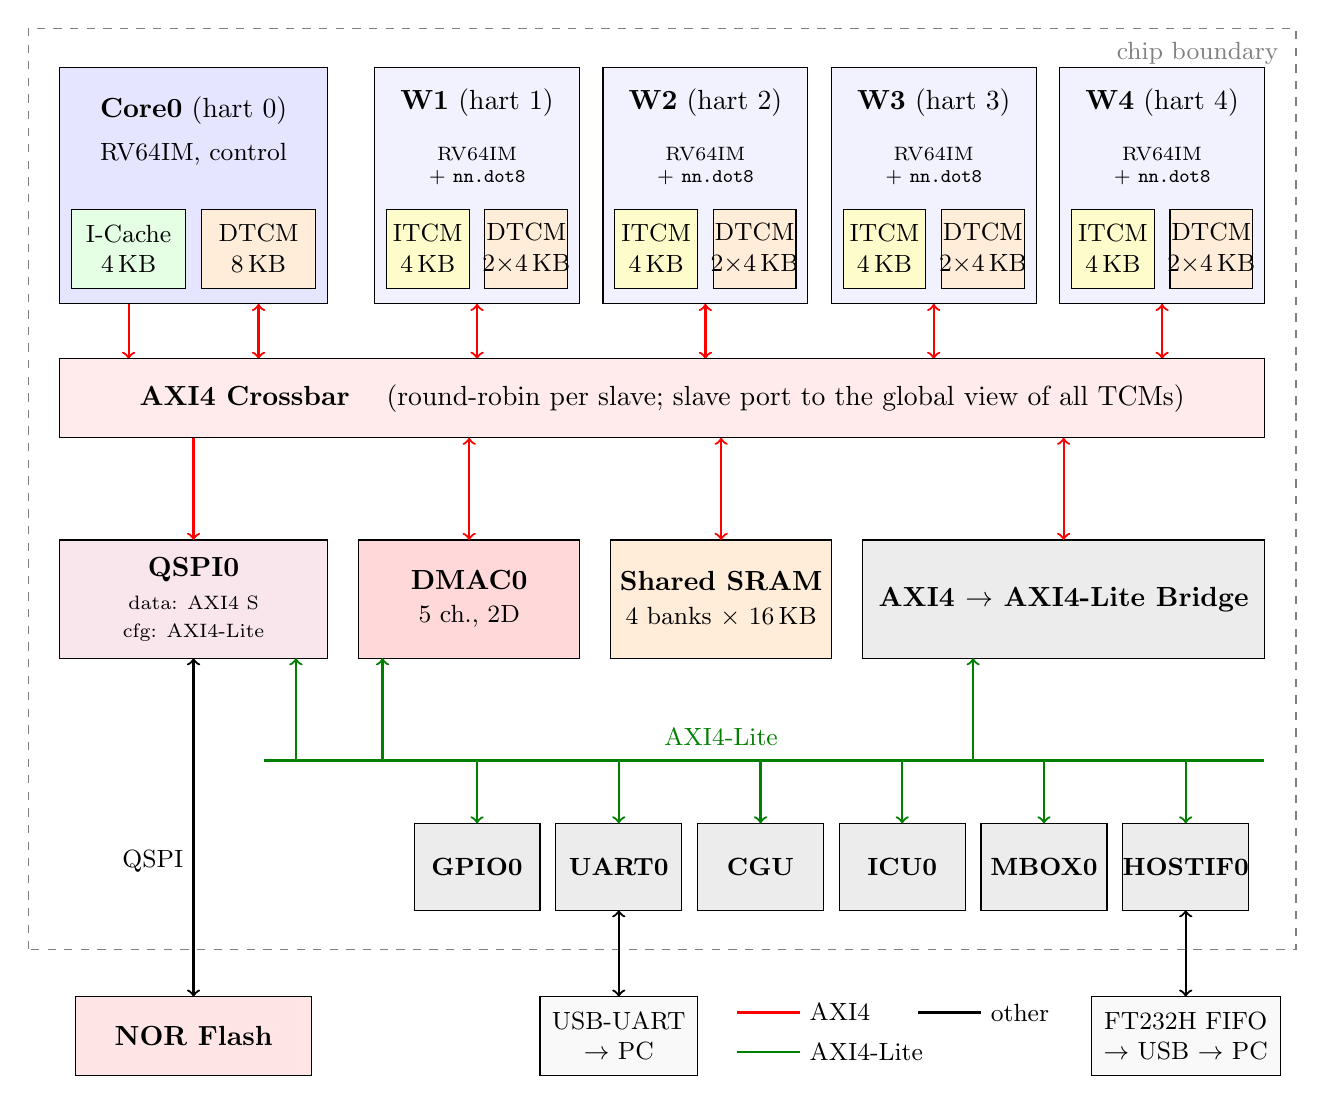
\begin{tikzpicture}[x=1cm, y=1cm]

  % ---- chip boundary ----
  \draw[dashed, gray] (-0.4,1.8) rectangle (15.7,13.5);
  \node[gray, font=\small, anchor=north east] at (15.6,13.45) {chip boundary};

  % ---- Core0 ----
  \filldraw[fill=blue!10, draw=black] (0.0,10.0) rectangle (3.4,13.0);
  \node[align=center] at (1.7,12.45) {\textbf{Core0} (hart 0)};
  \node[font=\small] at (1.7,11.9) {RV64IM, control};
  \filldraw[fill=green!10, draw=black] (0.15,10.2) rectangle (1.6,11.2);
  \node[font=\small, align=center] at (0.875,10.7) {I-Cache\\4\,KB};
  \filldraw[fill=orange!15, draw=black] (1.8,10.2) rectangle (3.25,11.2);
  \node[font=\small, align=center] at (2.525,10.7) {DTCM\\8\,KB};

  % ---- Workers ----
  \foreach \i/\x in {1/4.0, 2/6.9, 3/9.8, 4/12.7} {
    \filldraw[fill=blue!5, draw=black] (\x,10.0) rectangle (\x+2.6,13.0);
    \node at (\x+1.3,12.55) {\textbf{W\i} (hart \i)};
    \node[font=\scriptsize, align=center] at (\x+1.3,11.75) {RV64IM\\+ \texttt{nn.dot8}};
    \filldraw[fill=yellow!20, draw=black] (\x+0.15,10.2) rectangle (\x+1.2,11.2);
    \node[font=\small, align=center] at (\x+0.675,10.7) {ITCM\\4\,KB};
    \filldraw[fill=orange!15, draw=black] (\x+1.4,10.2) rectangle (\x+2.45,11.2);
    \node[font=\small, align=center] at (\x+1.925,10.7) {DTCM\\2$\times$4\,KB};
    \draw[thick, red, <->] (\x+1.3,10.0) -- (\x+1.3,9.3);
  }

  % ---- Core0 to crossbar: I-Cache (read) and data port ----
  \draw[thick, red, ->]  (0.875,10.0) -- (0.875,9.3);
  \draw[thick, red, <->] (2.525,10.0) -- (2.525,9.3);

  % ---- AXI4 crossbar ----
  \filldraw[fill=red!8, draw=black] (0.0,8.3) rectangle (15.3,9.3);
  \node at (7.65,8.8) {\textbf{AXI4 Crossbar} \quad (round-robin per slave; slave port to the global view of all TCMs)};

  % ---- slaves / masters below crossbar ----
  \filldraw[fill=purple!10, draw=black] (0.0,5.5) rectangle (3.4,7.0);
  \node[align=center] at (1.7,6.25) {\textbf{QSPI0}\\{\scriptsize data: AXI4 S}\\[-2pt]{\scriptsize cfg: AXI4-Lite}};
  \draw[thick, red, <-] (1.7,7.0) -- (1.7,8.3);

  \filldraw[fill=red!15, draw=black] (3.8,5.5) rectangle (6.6,7.0);
  \node[align=center] at (5.2,6.25) {\textbf{DMAC0}\\{\small 5 ch., 2D}};
  \draw[thick, red, <->] (5.2,7.0) -- (5.2,8.3);

  \filldraw[fill=orange!15, draw=black] (7.0,5.5) rectangle (9.8,7.0);
  \node[align=center] at (8.4,6.25) {\textbf{Shared SRAM}\\{\small 4 banks $\times$ 16\,KB}};
  \draw[thick, red, <->] (8.4,7.0) -- (8.4,8.3);

  \filldraw[fill=gray!15, draw=black] (10.2,5.5) rectangle (15.3,7.0);
  \node[align=center] at (12.75,6.25) {\textbf{AXI4 $\rightarrow$ AXI4-Lite Bridge}};
  \draw[thick, red, <->] (12.75,7.0) -- (12.75,8.3);

  % ---- AXI4-Lite peripheral bus ----
  \draw[thick, green!50!black] (2.6,4.2) -- (15.3,4.2);
  \node[green!50!black, font=\small] at (8.4,4.5) {AXI4-Lite};
  \draw[thick, green!50!black, <-] (11.6,5.5) -- (11.6,4.2);
  \draw[thick, green!50!black, ->] (4.1,4.2) -- (4.1,5.5);
  \draw[thick, green!50!black, ->] (3.0,4.2) -- (3.0,5.5);

  \foreach \n/\x in {GPIO0/5.3, UART0/7.1, CGU/8.9, ICU0/10.7, MBOX0/12.5, HOSTIF0/14.3} {
    \filldraw[fill=gray!15, draw=black] (\x-0.8,2.3) rectangle (\x+0.8,3.4);
    \node[font=\small] at (\x,2.85) {\textbf{\n}};
    \draw[thick, green!50!black, ->] (\x,4.2) -- (\x,3.4);
  }

  % ---- off-chip ----
  \filldraw[fill=red!10, draw=black] (0.2,0.2) rectangle (3.2,1.2);
  \node at (1.7,0.7) {\textbf{NOR Flash}};
  \draw[thick, <->] (1.7,5.5) -- (1.7,1.2) node[pos=0.6, left, font=\small]{QSPI};

  \filldraw[fill=gray!5, draw=black] (6.1,0.2) rectangle (8.1,1.2);
  \node[font=\small, align=center] at (7.1,0.7) {USB-UART\\$\rightarrow$ PC};
  \draw[thick, <->] (7.1,2.3) -- (7.1,1.2);

  \filldraw[fill=gray!5, draw=black] (13.1,0.2) rectangle (15.5,1.2);
  \node[font=\small, align=center] at (14.3,0.7) {FT232H FIFO\\$\rightarrow$ USB $\rightarrow$ PC};
  \draw[thick, <->] (14.3,2.3) -- (14.3,1.2);

  % ---- legend ----
  \draw[thick, red] (8.6,1.0) -- (9.4,1.0);
  \node[right, font=\small] at (9.4,1.0) {AXI4};
  \draw[thick, green!50!black] (8.6,0.5) -- (9.4,0.5);
  \node[right, font=\small] at (9.4,0.5) {AXI4-Lite};
  \draw[thick] (10.9,1.0) -- (11.7,1.0);
  \node[right, font=\small] at (11.7,1.0) {other};

\end{tikzpicture}}
\caption{Variant C -- Block Diagram (proposal)}
\label{fig:mcnnblock}
\end{figure}

\begin{table}[H]
\caption{Variant C -- Building Blocks}
\label{tab:mcnnblocks}
\centering
{\footnotesize
\begin{tabularx}{\textwidth}{|p{0.2\textwidth} |p{0.3\textwidth} |X|}
  \hline
  Block & Origin & Function in Variant C \\
  \hline
  \hline
  Core0 & \texttt{cc\_cpupipefwd} + M & Boot from Flash (XIP), host protocol,
    layer scheduling, requantisation of partial results if required \\
  \hline
  W1\ldots W4 & \texttt{cc\_cpupipefwd} + M + \texttt{nn.dot8} &
    NN kernels (fully connected, convolution, activation) on tiles in the DTCM \\
  \hline
  I-Cache (Core0) & Variant~B, unchanged & XIP from NOR Flash via QSPI0 \\
  \hline
  ITCM / DTCM & new (SPRAM macros) & Private single-cycle memories \\
  \hline
  Shared SRAM & new (SPRAM macros) & Weights, activations, messages \\
  \hline
  AXI4 crossbar & new & Memory interconnect, 7 masters, 4 slave groups \\
  \hline
  AXI4$\rightarrow$AXI4-Lite bridge & new & Peripheral access \\
  \hline
  DMAC0 & new & 2D tile transfers Flash/SRAM/TCM \\
  \hline
  MBOX0 & new & Hart release, IPIs, semaphores, message registers \\
  \hline
  HOSTIF0 & new & FT232H synchronous FIFO interface \\
  \hline
  QSPI0, UART0, GPIO0, CGU, ICU0 & existing & Bus front end changed from
    Wishbone to AXI4-Lite; kernels unchanged \\
  \hline
  \texttt{as\_irq\_peripheral} & existing & Interrupt registers of DMAC0,
    MBOX0 and HOSTIF0 \\
  \hline
\end{tabularx}}
\end{table}

%=============================================================
% Core
%=============================================================
\section{Core Extensions}
\label{sec:mcnncore}

All five cores are instances of \texttt{cc\_cpupipefwd}
(Section~``RWU-RV64I Core'' and Section~\ref{subsec:chipVariants}) with
the extensions of this section.
The 5-stage pipeline with forwarding is kept.

\subsection{M Extension}
\label{subsec:mcnnmext}

The M extension is implemented as a multi-cycle unit in the EX stage that
stalls the pipeline until the result is available (MCNN-CO-002).
A radix-4 iterative multiplier needs 32 cycles for $64\times64$ bit plus
setup; a radix-2 restoring divider needs 64 cycles plus setup.
A fully combinational $64\times64$ multiplier is not recommended: in a
350\,nm process it would dominate both the area and the critical path.

The low performance of MUL is acceptable because the NN inner loop does not
use it (see Section~\ref{subsec:mcnnperf}): MUL is used once per output
value for requantisation, i.e.\ once per several hundred MACs.

\subsection{Custom Instruction \texttt{nn.dot8}}
\label{subsec:mcnndot8}

\texttt{nn.dot8} interprets both source registers as vectors of eight
signed 8-bit values and returns the sum of the eight products:
\[
  \texttt{rd} = \sum_{i=0}^{7}
     \operatorname{sext}\!\left(\texttt{rs1}[8i{+}7:8i]\right) \cdot
     \operatorname{sext}\!\left(\texttt{rs2}[8i{+}7:8i]\right)
\]
The result range is $|\texttt{rd}| \leq 8 \cdot 128 \cdot 128 = 131\,072$
(19 bit signed); it is sign-extended to 64 bit.
The instruction uses the R-type format in the \texttt{custom-0} opcode
space reserved by the RISC-V specification for vendor extensions
(Table~\ref{tab:mcnndot8enc}).

\begin{table}[H]
\caption{Encoding of the NN Custom Instructions (opcode \texttt{custom-0} = \texttt{0001011})}
\label{tab:mcnndot8enc}
\centering
{\footnotesize
\begin{tabularx}{\textwidth}{|l |l |l |X|}
  \hline
  Mnemonic & funct7 & funct3 & Operation / Status \\
  \hline
  \hline
  \texttt{nn.dot8 rd, rs1, rs2}  & \texttt{0000000} & \texttt{000} &
    signed $\times$ signed, 8 lanes; \textbf{mandatory} for workers \\
  \hline
  \texttt{nn.dot8su rd, rs1, rs2} & \texttt{0000000} & \texttt{001} &
    signed (\texttt{rs1}) $\times$ unsigned (\texttt{rs2}); \textit{optional},
    for unsigned activations after ReLU \\
  \hline
  \texttt{nn.dot8a rd, rs1, rs2} & \texttt{0000000} & \texttt{010} &
    \texttt{rd += dot8(rs1, rs2)}; \textit{optional}, requires a third
    register-file read port \\
  \hline
  \texttt{nn.clip8 rd, rs1, rs2} & \texttt{0000000} & \texttt{011} &
    saturate \texttt{rs1} to $[-128, 127]$, then ReLU if \texttt{rs2}[0]\,=\,1;
    \textit{optional} \\
  \hline
\end{tabularx}}
\end{table}

\textbf{Why no accumulating variant in the first version:} an accumulating
instruction reads \texttt{rd} as a third operand. The register file of
\texttt{cc\_cpupipefwd} has two read ports, and the forwarding network would
need a third path. The non-accumulating \texttt{nn.dot8} followed by an
\texttt{add} costs one instruction more per 8 MACs and fits the existing
data path unchanged.

\textbf{Implementation:} eight $8\times8$ signed multipliers and an adder
tree in the EX stage. If the path does not close timing in one cycle in the
target process, \texttt{nn.dot8} \textit{may} take two cycles (products
registered, pipeline stalled for one cycle). The decoder treats all other
\texttt{funct3}/\texttt{funct7} values of \texttt{custom-0} as illegal
instructions.

\textbf{Tool support:} the GNU assembler accepts the instruction without a
toolchain change via
\texttt{.insn r 0x0B, 0, 0, rd, rs1, rs2}; a C intrinsic is a one-line
inline-assembly macro.

\subsection{CSRs, Interrupts and Reset Vector}
\label{subsec:mcnncsr}

\begin{itemize}
  \item \texttt{mhartid} (\texttt{0xF14}, read-only): parameter
    \texttt{HART\_ID}, 0 for Core0, 1\ldots4 for the workers (MCNN-CO-004).
  \item \texttt{mip.MSIP} / \texttt{mie.MSIE} (bit~3): software interrupt,
    driven by MBOX0 (MCNN-CO-005), cause code \texttt{0x8000\ldots0003}.
  \item \texttt{mip.MEIP} (bit~11): Core0: \texttt{icu\_irq\_o} of ICU0 as in
    Variants~A/B. Workers: interrupt of their own DMA channel.
  \item Reset vector: parameter \texttt{RESET\_PC}; Core0: Flash base,
    workers: local ITCM base (MCNN-CO-006).
\end{itemize}

%=============================================================
% Memory architecture
%=============================================================
\section{Memory Architecture}
\label{sec:mcnnmem}

\subsection{Why the Workers Have No Caches}
\label{subsec:mcnnnocache}

NN inference has a static data access pattern: which weights and which
activations are needed at which time is known before the program runs.
A cache would guess what the software already knows. Table~\ref{tab:mcnncachetcm}
compares both options for the worker cores.

\begin{table}[H]
\caption{D-Cache versus DTCM for the Worker Cores}
\label{tab:mcnncachetcm}
\centering
{\footnotesize
\begin{tabularx}{\textwidth}{|l |X |X|}
  \hline
   & D-Cache (as in Variant~B) & DTCM (Variant~C) \\
  \hline
  \hline
  Coherence between 4 cores & required (snooping/directory) or flush by software & not required, private memory \\
  \hline
  Access time & hit/miss, not deterministic & always 1 cycle \\
  \hline
  Area & tag SRAM, PLRU, refill FSM, AXI4 master & SRAM macro and address decoder only \\
  \hline
  Usable capacity & reduced by conflict misses & 100\,\% \\
  \hline
  Data movement & implicit (refills) & explicit (DMA), plannable, overlaps with compute \\
  \hline
  Software effort & none & tiling and double buffering in the NN runtime \\
  \hline
\end{tabularx}}
\end{table}

A DTCM access behaves like a cache access that always hits.
The 1-cycle load-use stall of \texttt{cc\_cpupipefwd} remains; the stall
logic for cache misses is not used for TCM addresses.

The workers execute only small, fixed kernels (a few KB of code).
Core0 loads them into the ITCMs before releasing the workers
(MCNN-SN-003); an I-Cache is therefore not needed either.
Core0 keeps its I-Cache because it executes general code in place from the
NOR Flash.

\subsection{Address Map (proposal)}
\label{subsec:mcnnaddrmap}

The address map keeps the convention of Variants~A/B: bit~32\,=\,1 selects
the peripheral bus (Table~\ref{tab:sysmap}).

\begin{table}[H]
\caption{Variant C -- Address Map (proposal)}
\label{tab:mcnnaddrmap}
\centering
{\scriptsize
\begin{tabularx}{\textwidth}{|p{0.25\textwidth} |p{0.09\textwidth} |p{0.17\textwidth} |X|}
  \hline
  Base Address & Size & Region & Notes \\
  \hline
  \hline
  \texttt{0x0000\_0000\_0000\_0000} & 16\,MB & NOR Flash (XIP) &
    Read-only. Cached by the I-Cache of Core0; DMA source for weights.
    Reset vector of Core0. \\
  \hline
  \texttt{0x0000\_0000\_1000\_0000} & 64\,KB & Shared SRAM &
    4 banks $\times$ 16\,KB, interleaved on address bit~3 and~4
    (consecutive doublewords in different banks). Uncached. \\
  \hline
  \texttt{0x0000\_0000\_2000\_0000} & 4\,KB & ITCM (local alias) &
    Each worker sees its own ITCM. Reset vector of the workers.
    Not present in Core0. \\
  \hline
  \texttt{0x0000\_0000\_2001\_0000} & 2 $\times$ 4\,KB & DTCM (local alias) &
    Bank~0 at \texttt{+0x0000}, bank~1 at \texttt{+0x1000}.
    Core0: 8\,KB DTCM (stack, \texttt{.data}, \texttt{.bss}). \\
  \hline
  \texttt{0x0000\_0000\_3000\_0000}\newline + $h \cdot$\texttt{0x0010\_0000} & 1\,MB each & TCMs of hart $h$ (global) &
    ITCM at \texttt{+0x0\_0000}, DTCM at \texttt{+0x1\_0000};
    $h = 0\ldots4$. Used by DMAC0 and Core0. \\
  \hline
  \texttt{0x0000\_0001\_0000\_0000} & 2.5\,KB & GPIO0, QSPI0 cfg, CGU, UART0, ICU0 &
    Unchanged offsets of Table~\ref{tab:sysmap}. \\
  \hline
  \texttt{0x0000\_0001\_0000\_0A00} & 512\,B & DMAC0 & Table~\ref{tab:mcnndmaregs}. \\
  \hline
  \texttt{0x0000\_0001\_0000\_0C00} & 512\,B & MBOX0 & Table~\ref{tab:mcnnmboxregs}. \\
  \hline
  \texttt{0x0000\_0001\_0000\_0E00} & 512\,B & HOSTIF0 & Section~\ref{sec:mcnnext}. \\
  \hline
\end{tabularx}}
\end{table}

\subsection{Memory Sizes and Area}
\label{subsec:mcnnsizes}

Table~\ref{tab:mcnnsram} lists the proposed SRAM instances. All sizes are
parameters; the values are chosen so that an MNIST MLP with
784--64--10 neurons (50\,816 int8 weights, Section~\ref{subsec:mcnnperf})
fits completely into the shared SRAM.

\begin{table}[H]
\caption{Variant C -- SRAM Instances (proposal)}
\label{tab:mcnnsram}
\centering
{\footnotesize
\begin{tabularx}{\textwidth}{|l |l |l |l |X|}
  \hline
  Instance & Organisation & Count & Total & Notes \\
  \hline
  \hline
  ITCM (W1\ldots W4) & $64 \times 512$ & 4 & 16\,KB & \\
  \hline
  DTCM bank (W1\ldots W4) & $64 \times 512$ & 8 & 32\,KB & 2 banks per worker \\
  \hline
  DTCM (Core0) & $64 \times 1024$ & 1 & 8\,KB & as Scratchpad in Variant~B \\
  \hline
  I-Cache (Core0) & as Variant~B & 1+1 & 4.4\,KB & data + tag \\
  \hline
  Shared SRAM bank & $64 \times 2048$ & 4 & 64\,KB & \\
  \hline
  \multicolumn{3}{|l|}{\textbf{Total}} & \textbf{$\approx$124\,KB} & \\
  \hline
\end{tabularx}}
\end{table}

\textbf{Area is the critical resource.} In the XH035 process
(Section~\ref{subsec:sramSelection}) SRAM macros are large; the total area
of Table~\ref{tab:mcnnsram} must be estimated with the SPRAM compiler before
the sizes are frozen (open issue MCNN-OI-01). The first reduction steps are,
in this order: \texttt{NR\_WORKERS}\,=\,2, shared SRAM 32\,KB (weights
streamed from Flash by DMA), DTCM banks 2\,KB.

\subsection{Double Buffering}
\label{subsec:mcnnpingpong}

The XH035 SPRAM macros have a single port. A DMA write and a core access to
the same macro therefore exclude each other. Each worker DTCM is split into
two macros (banks) which are used alternately:

\begin{center}
{\footnotesize
\begin{tabular}{|l |l |l|}
  \hline
  Phase & Core computes on & DMA fills \\
  \hline
  $2k$   & bank 0 (tile $2k$)   & bank 1 (tile $2k{+}1$) \\
  \hline
  $2k{+}1$ & bank 1 (tile $2k{+}1$) & bank 0 (tile $2k{+}2$) \\
  \hline
\end{tabular}}
\end{center}

If software nevertheless accesses a bank that the DMA is writing, the core
access wins (MCNN-IC-004) and the DMA is delayed; the result stays correct.
The worker waits for the DMA completion interrupt (or polls the channel
status) before it switches to the next bank.

\subsection{Rules for Shared Data}
\label{subsec:mcnnshared}

Because there is no data cache anywhere, the only coherence rules are:
\begin{enumerate}
  \item A buffer is written by exactly one agent (one core or one DMA channel)
    at a time; ownership is passed by a semaphore, a message register or an
    IPI (Section~\ref{sec:mcnnsync}).
  \item Before ownership is passed, the writer issues a \texttt{FENCE}; the
    core waits for the B response of all outstanding AXI4 writes.
  \item The I-Cache of Core0 is invalidated with \texttt{FENCE.I} after the
    Flash content has been changed (programming over the host interface).
\end{enumerate}

%=============================================================
% Interconnect
%=============================================================
\section{Interconnect}
\label{sec:mcnnic}

\subsection{AXI4 Crossbar}
\label{subsec:mcnnxbar}

\begin{table}[H]
\caption{AXI4 Crossbar -- Masters and Slaves}
\label{tab:mcnnxbar}
\centering
{\footnotesize
\begin{tabularx}{\textwidth}{|l |l |X|}
  \hline
  Port & Block & Notes \\
  \hline
  \hline
  M0 & Core0 I-Cache & Read only, 4-beat bursts (as Variant~B) \\
  \hline
  M1 & Core0 data port & Single beats; shared SRAM, TCMs (global), peripherals \\
  \hline
  M2\ldots M5 & W1\ldots W4 data port & Single beats; local TCM accesses do \emph{not} use the crossbar \\
  \hline
  M6 & DMAC0 & Bursts up to 16 beats, read and write \\
  \hline
  \hline
  S0 & QSPI0 data port & Read only (Flash) \\
  \hline
  S1\ldots S4 & Shared SRAM banks 0\ldots3 & 1 beat per cycle each \\
  \hline
  S5 & TCM global port & Routes to the ITCM/DTCM bank of hart $h$; lower priority than the owning core \\
  \hline
  S6 & AXI4$\rightarrow$AXI4-Lite bridge & All peripherals \\
  \hline
\end{tabularx}}
\end{table}

Parameters: data width 64\,bit, address width 33\,bit (bit~32 selects
the peripherals), ID width 4\,bit (master number). Each master has at most
one outstanding transaction per direction in the first version.

\textbf{Bandwidth check:} with \texttt{nn.dot8} a worker needs about one byte
of weights per cycle (8 bytes per 8 MACs, Section~\ref{subsec:mcnnperf}).
Four workers need about 4\,B/cycle; four shared SRAM banks deliver up to
32\,B/cycle. The shared SRAM is therefore not the bottleneck; the DMA
controller with one master port (8\,B/cycle) is sufficient as long as the
input activations are reused from the DTCM.

\subsection{Peripheral Bus AXI4-Lite}
\label{subsec:mcnnperbus}

The peripheral kernels and the shared interrupt register block are
connected to the Wishbone slave BPI \texttt{as\_slave\_bpi}
(Section~\ref{subsec:asSlaveBpi}) via its kernel-side signals
(\texttt{addr\_o}, \texttt{wr\_o}, data). Variant~C replaces only the bus side:
a new BPI \texttt{cc\_axil\_slave\_bpi} implements an AXI4-Lite slave and
provides the \emph{same} kernel-side signals. The peripheral kernels and
\texttt{as\_irq\_peripheral} remain unchanged.

QSPI0 keeps its dual role (Section~\ref{subsec:asAxi4Bus}): data port on
AXI4, configuration on the peripheral bus, now AXI4-Lite.

%=============================================================
% DMA
%=============================================================
\section{DMA Controller DMAC0}
\label{sec:mcnndma}

DMAC0 has one AXI4 master port and one AXI4-Lite configuration port.
It provides \texttt{NR\_WORKERS}+1 channels (MCNN-DM-001); the channels are
served round-robin, one burst at a time.
Each channel copies a 2D block:
\[
  \text{for } r = 0 \ldots \text{ROWS}{-}1:\quad
  \text{copy LEN bytes from } \text{SRC} + r\cdot\text{SSTRIDE}
  \text{ to } \text{DST} + r\cdot\text{DSTRIDE}
\]
SRC, DST, LEN and the strides must be multiples of 8 (doubleword transfers
only); otherwise the channel reports an error and does not start.

\begin{table}[H]
\caption{DMAC0 Registers (proposal; channel $c$ at offset $c \cdot$\texttt{0x40})}
\label{tab:mcnndmaregs}
\centering
{\footnotesize
\begin{tabularx}{\textwidth}{|l |l |l |X|}
  \hline
  Offset & Name & Mode & Description \\
  \hline
  \hline
  \texttt{0x00} & SRC     & rw & Source address \\
  \hline
  \texttt{0x08} & DST     & rw & Destination address \\
  \hline
  \texttt{0x10} & LEN     & rw & Bytes per row \\
  \hline
  \texttt{0x18} & ROWS    & rw & Number of rows (1 = 1D transfer) \\
  \hline
  \texttt{0x20} & SSTRIDE & rw & Source row stride in bytes \\
  \hline
  \texttt{0x28} & DSTRIDE & rw & Destination row stride in bytes \\
  \hline
  \texttt{0x30} & CTRL    & w  & Bit 0: START (write-1 strobe); ignored while BUSY \\
  \hline
  \texttt{0x38} & STATUS  & r  & Bit 0: BUSY; bit 1: ERROR (alignment or AXI error response) \\
  \hline
  \hline
  \texttt{0x180}\ldots & IMSC, RIS, MIS, ICR, ISR & & \texttt{as\_irq\_peripheral}
    with \texttt{irqs\_yes\_no}\,=\,0: RIS[$c$] = channel $c$ done,
    RIS[$8{+}c$] = channel $c$ error \\
  \hline
\end{tabularx}}
\end{table}

\textbf{Interrupts:} the done and error bits of channel~$h$ ($h \geq 1$) are
routed to \texttt{mip.MEIP} of worker~$h$; channel~0 is routed to ICU0
(Core0). For this per-hart routing DMAC0 provides one masked interrupt
output per channel in addition to the combined \texttt{irq\_o} of the
shared block.

%=============================================================
% Synchronisation
%=============================================================
\section{Synchronisation and Inter-Processor Interrupts}
\label{sec:mcnnsync}

The cores do not implement the A extension (atomics). Mutual exclusion and
signalling are provided by the peripheral MBOX0 instead. Its registers are
uncached and every access is a single, non-speculative bus transaction,
so a read with a side effect is safe.

\begin{table}[H]
\caption{MBOX0 Registers (proposal)}
\label{tab:mcnnmboxregs}
\centering
{\footnotesize
\begin{tabularx}{\textwidth}{|l |l |l |X|}
  \hline
  Offset & Name & Mode & Description \\
  \hline
  \hline
  \texttt{0x000} & HART\_RUN & rw & Bit $h$\,=\,1 releases worker $h$ from its
    inactive state; it then starts at its reset vector. Bit 0 (Core0) reads 1. \\
  \hline
  \texttt{0x008} & IPI\_SET & w & Write-1 strobe: sets MSIP of hart $h$ for every bit $h$ written as 1 \\
  \hline
  \texttt{0x010} & IPI\_CLR & w & Write-1 strobe: clears MSIP of hart $h$ \\
  \hline
  \texttt{0x018} & IPI\_PEND & r & Current MSIP state of all harts \\
  \hline
  \texttt{0x040} + $8s$ & SEM$s$ & r/w & Semaphore $s = 0\ldots7$.
    \textbf{Read} returns the old value (0\,=\,was free) and sets the
    semaphore to 1 (test-and-set). \textbf{Write} 0 releases it. \\
  \hline
  \texttt{0x100} + $8h$ & MSG$h$ & rw & Message register of hart $h$
    (e.g.\ pointer to a job descriptor) \\
  \hline
\end{tabularx}}
\end{table}

\textbf{Lock:} \texttt{while (MBOX0\_SEM[s] != 0) ;} \ldots critical section
\ldots \texttt{FENCE; MBOX0\_SEM[s] = 0;}

\textbf{Arbitration:} the AXI4-Lite bridge serialises the accesses, so two
simultaneous reads of the same free semaphore are executed one after the
other; exactly one core reads 0.

The MSIP bits are not stored in \texttt{as\_irq\_peripheral}: each bit
drives the MSIP input of one hart directly and stays set until the
receiving hart clears it via IPI\_CLR (level-sensitive software
interrupt, as defined by the RISC-V privileged specification).

%=============================================================
% External interfaces
%=============================================================
\section{External Interfaces}
\label{sec:mcnnext}

\begin{table}[H]
\caption{Host Interface Options}
\label{tab:mcnnhostif}
\centering
{\footnotesize
\begin{tabularx}{\textwidth}{|l |l |l |X|}
  \hline
  Interface & Throughput & Pins & Assessment \\
  \hline
  \hline
  UART0 (existing) & $\approx$100\,KB/s at 1\,Mbit/s & 2 &
    Control, debug, small inputs (one MNIST image, 784\,B, in $\approx$8\,ms). \\
  \hline
  SPI slave & several MB/s & 4 & Simple; PC side needs a USB-SPI bridge. \\
  \hline
  \textbf{FT232H sync.\ FIFO} & 10--40\,MB/s & 13 &
    \textbf{Recommended} (HOSTIF0). Digital 8-bit FIFO with
    \texttt{RXF\#}, \texttt{TXE\#}, \texttt{RD\#}, \texttt{WR\#}, \texttt{OE\#}
    and a 60\,MHz clock from the FT232H; USB to the PC via the vendor driver. \\
  \hline
  Ethernet RMII & 100\,Mbit/s & 9 & Needs an external PHY and a network stack on Core0. \\
  \hline
  PCIe & $\geq$250\,MB/s & -- & Not possible in the ASIC (MCNN-IF-003); FPGA prototype only. \\
  \hline
\end{tabularx}}
\end{table}

\textbf{HOSTIF0} contains a receive and a transmit FIFO (reuse of
\texttt{as\_fifo}) with a clock domain crossing to the 60\,MHz FIFO clock of
the FT232H, an AXI4-Lite register interface and interrupts via
\texttt{as\_irq\_peripheral}. A DMA channel can move data between its FIFOs
and the shared SRAM.

The NOR Flash holds the boot code of Core0, the worker kernels and the NN
weights. With 50\,MHz Quad SPI the Flash delivers about 25\,MB/s; weights
are therefore copied once into the shared SRAM at start-up and are not
streamed during inference (unless the area reduction of
Section~\ref{subsec:mcnnsizes} requires it).

%=============================================================
% Software model and performance
%=============================================================
\section{Software Model and Performance}
\label{sec:mcnnsw}

\subsection{Boot and Inference Flow}
\label{subsec:mcnnflow}

\begin{enumerate}
  \item Reset: Core0 starts from Flash (XIP via I-Cache); the workers are
    inactive (MCNN-SN-003).
  \item Core0 copies the worker kernels from Flash into the four ITCMs and
    the NN weights into the shared SRAM (DMA channel 0), then sets
    MBOX0\_HART\_RUN.
  \item The workers initialise their stack in the DTCM, enable MSIP and wait
    for an IPI.
  \item Core0 receives an input (UART0 or HOSTIF0) into the shared SRAM.
  \item For each layer Core0 writes one job descriptor per worker (layer type,
    addresses, output range) and sends an IPI to every worker.
  \item Each worker copies the input activations into its DTCM, then
    processes its share of the outputs tile by tile with double buffering,
    writes the outputs into the shared SRAM, executes \texttt{FENCE} and
    signals completion (IPI to Core0 or semaphore counter).
  \item After the last layer Core0 sends the result to the host.
\end{enumerate}

\textbf{Work partitioning:} fully connected layers are split by output
neurons, convolution layers by output channels. Each worker then needs the
complete input but only its own rows of the weight matrix; no partial sums
have to be combined across workers.

\textbf{Quantisation:} int8 weights and activations (symmetric), int32
accumulators, bias as int32. Requantisation per output:
$y = \operatorname{clip}_{[-128,127]}\!\left((acc \cdot M) \gg s\right)$
with a per-layer integer multiplier $M$ and shift $s$ (one MUL per output).

\subsection{Performance Estimate}
\label{subsec:mcnnperf}

Inner loop of a fully connected layer with \texttt{nn.dot8}, unrolled
twice (16 MACs):

\begin{lstlisting}[basicstyle=\ttfamily\footnotesize, frame=single]
loop: ld      a0, 0(s0)        # 8 weights
      ld      a1, 0(s1)        # 8 activations
      ld      a2, 8(s0)
      ld      a3, 8(s1)
      nn.dot8 t0, a0, a1
      nn.dot8 t1, a2, a3
      add     s2, s2, t0
      add     s2, s2, t1
      addi    s0, s0, 16
      addi    s1, s1, 16
      bne     s0, s3, loop
\end{lstlisting}

11 instructions per 16 MACs; with the load instructions scheduled ahead of
their use there is no load-use stall, so with one taken-branch penalty the
loop needs about 13 cycles, i.e.\ $\approx$0.8 cycles per MAC.

\begin{table}[H]
\caption{Performance Estimate per Worker (int8 MAC)}
\label{tab:mcnnperf}
\centering
{\footnotesize
\begin{tabularx}{\textwidth}{|l |l |X|}
  \hline
  Implementation & Cycles / MAC & Remark \\
  \hline
  \hline
  RV64I, multiplication in software & $\approx$ 100--200 & shift-and-add loop per product (TBD) \\
  \hline
  RV64IM, iterative MUL (MCNN-CO-002) & $\approx$ 40 & 34 cycles MUL + loads + add \\
  \hline
  RV64IM + \texttt{nn.dot8} & $\approx$ 0.8 & loop above \\
  \hline
  RV64IM + \texttt{nn.dot8a} (optional) & $\approx$ 0.6 & accumulate saves the two \texttt{add} \\
  \hline
\end{tabularx}}
\end{table}

With $f_\text{clk}$ as the system clock frequency (TBD for XH035, see
open issue MCNN-OI-02) the peak performance of four workers is
\[
  P \approx 4 \cdot \frac{f_\text{clk}}{0.8} = 5 \cdot f_\text{clk}
  \;\text{MAC/s}
  \qquad (\text{e.g. } 125\,\text{MMAC/s at } 25\,\text{MHz}).
\]

\begin{table}[H]
\caption{Example Networks (4 workers, \texttt{nn.dot8}, $f_\text{clk} = 25$\,MHz, compute time only)}
\label{tab:mcnnnets}
\centering
{\footnotesize
\begin{tabularx}{\textwidth}{|l |l |l |X|}
  \hline
  Network & MACs & Weights (int8) & Time \\
  \hline
  \hline
  MNIST MLP 784--64--10 & 51\,k & 51\,KB & $\approx$0.4\,ms -- fits the shared SRAM \\
  \hline
  LeNet-5 & 0.4\,M & 62\,KB & $\approx$3\,ms \\
  \hline
  Keyword spotting (DS-CNN small) & 2.7\,M & 39\,KB & $\approx$22\,ms \\
  \hline
  MobileNet V1 0.25 (128$\times$128) & 14\,M & 470\,KB & $\approx$0.1\,s, weights must be streamed from Flash \\
  \hline
\end{tabularx}}
\end{table}

The values are estimates for the compute time of the inner loops; DMA
waiting time, synchronisation and requantisation add an overhead that is
determined in simulation (milestone M4, Table~\ref{tab:mcnnroadmap}).

%=============================================================
% Verification
%=============================================================
\section{Verification Strategy}
\label{sec:mcnnverif}

\begin{itemize}
  \item \textbf{Instruction level:} the ISS scoreboard of the cocotb
    environment (Section~\ref{sec:simtest01}) is extended by the M
    extension and \texttt{nn.dot8}; the RISC-V architectural tests for
    \texttt{rv64im} are added to the regression. Random operands for
    \texttt{nn.dot8} cover the corner cases $-128 \cdot -128$ in all lanes.
  \item \textbf{Block level:} DMAC0 (2D addressing, alignment errors,
    arbitration against the owning core), MBOX0 (semaphore contention of
    five harts, IPI), crossbar (round-robin, no starvation),
    \texttt{cc\_axil\_slave\_bpi} (protocol checker).
  \item \textbf{System level:} boot from the Flash model, release of the
    workers, ping-pong DMA, one complete MNIST inference.
    The output of every layer is compared bit-exactly with a
    Python/NumPy integer reference model (MCNN-VE-002).
  \item \textbf{Prototype:} FPGA implementation before tapeout; here the
    host interface may additionally be tested with PCIe hard IP.
\end{itemize}

%=============================================================
% Roadmap and open issues
%=============================================================
\section{Roadmap}
\label{sec:mcnnroadmap}

\begin{table}[H]
\caption{Variant C -- Milestones}
\label{tab:mcnnroadmap}
\centering
{\footnotesize
\begin{tabularx}{\textwidth}{|l |X |X|}
  \hline
  Milestone & Content & Exit criterion \\
  \hline
  \hline
  M1 & M extension in \texttt{cc\_cpupipefwd} (Variant~B) & \texttt{rv64im} architectural tests pass; xsim and cocotb regression green \\
  \hline
  M2 & \texttt{nn.dot8}, \texttt{mhartid}, MSIP & MNIST MLP on one core (Variant~B) bit-exact against the reference model \\
  \hline
  M3 & AXI4 with write channels, crossbar, AXI4-Lite bridge, \texttt{cc\_axil\_slave\_bpi} & All Variant~B tests pass on the new bus \\
  \hline
  M4 & TCMs, DMAC0, MBOX0, multi-core top level & MNIST MLP on four workers; overhead measured \\
  \hline
  M5 & HOSTIF0, FPGA prototype & Inference requested from the PC \\
  \hline
  M6 (option) & Systolic array (e.g.\ $8\times8$ MAC) as AXI4 slave with DMA & Speed-up factor versus M4 \\
  \hline
\end{tabularx}}
\end{table}

\section{Open Issues}
\label{sec:mcnnopen}

\begin{table}[H]
\caption{Variant C -- Open Issues}
\label{tab:mcnnopen}
\centering
{\footnotesize
\begin{tabularx}{\textwidth}{|l |X|}
  \hline
  ID & Issue \\
  \hline
  \hline
  MCNN-OI-01 & Area of the SRAM macros of Table~\ref{tab:mcnnsram} in XH035;
    decide \texttt{NR\_WORKERS} and memory sizes. \\
  \hline
  MCNN-OI-02 & Achievable $f_\text{clk}$ in XH035 (critical paths: \texttt{nn.dot8}
    adder tree, crossbar, SRAM access time, Table~\ref{tab:asSramTiming}). \\
  \hline
  MCNN-OI-03 & Debug access to five harts (JTAG scan chain per hart or a
    debug module according to the RISC-V debug specification). \\
  \hline
  MCNN-OI-04 & Semaphores in MBOX0 versus A extension (\texttt{lr/sc},
    \texttt{amoadd}); the A extension would be required for standard
    multi-threaded C libraries. \\
  \hline
  MCNN-OI-05 & Crossbar versus a shared AXI4 bus with arbiter
    (area versus bandwidth); decision after the simulation of M4. \\
  \hline
  MCNN-OI-06 & Power: clock gating of idle workers requires a real
    \texttt{WFI} (MCNN-CO-007). \\
  \hline
\end{tabularx}}
\end{table}
